Dựa trên các cơ sở lý thuyết tại chương I, chương này của luận văn trình bày về
phương pháp nghiên cứu và phát triển hệ thống thu thập, xử lý và lưu trữ dữ
liệu cảm biến gia tốc. Từ bộ dữ liệu thu thập, sẽ tiến hành trích xuất đặc
trưng, đề xuất mô hình học máy phù hợp và thiết lập các kịch bản để đánh giá
các mô hình đề xuất đó.
\section{Nghiên cứu, phát triển phần cứng }

\subsection{Vi điều khiển}
\label{subsec:vi_xu_ly}
Trong khuôn khổ luận văn sẽ sử dụng vi điều khiển
nRF52840 làm bộ điều khiển trung tâm.
Vi điều khiển này được trang bị bộ nhớ 1~MB Flash và 256~kb RAM phù hợp để
triển khai các mô hình cho bài toán phân loại tư thế ngủ.

\subsection{Cảm biến}
\label{subsec:cam_bien}

Sau khi đã khảo sát, cảm biến gia tốc Bosch BMI270 được lựa chọn cho hệ thống
nhận diện tư thế ngủ bao gồm các lý do: độ chính xác và dải đo linh hoạt, mức
tiêu thụ năng lượng thấp, tốc độ lấy mẫu, khả năng chống nhiễu.

\subsection{Bluetooth năng lượng thấp}

BLE được lựa chọn làm chuẩn kết nối không dây chính trong hệ thống phần cứng.
So với các giao thức khác, BLE tỏ ra vượt trội nhờ mức tiêu thụ năng lượng rất
thấp, tốc độ khởi tạo kết nối nhanh và khả năng tương thích rộng rãi với hầu
hết các thiết bị di động hiện nay. BLE tổ chức logic giao tiếp dựa trên mô hình
hồ sơ thuộc tính tổng quá \gls{gatt}.

\subsection{Thiết kế mạch}

Để đảm bảo các yêu cầu đặt ra, hệ thống cần
các khối sau: 01) Khối điều khiển: có chức năng xử lý toàn bộ logic trong
mạch, kết nối được với các thiết bị khác như điện thoại thông qua BLE và đặc
biệt, đủ hiệu năng để triển khai các mô hình học máy; 02) Khối cảm biến: có
nhiệm vụ thu thập dữ liệu sinh lý bao gồm 2 cảm biến chính là gia tốc (đã được
trình bày các phần trên) và thêm cảm biến âm thanh để phục vụ bài toán xác định
tiếng ngáy của nhóm; 03) Khối nguồn: có nhiệm vụ ổn áp về đúng dải điện áp
tương thích, lọc nhiễu, bảo vệ dòng; 04) Khối nạp và gỡ lỗi: có nhiệm vụ nạp mã
chương trình vào vi điều khiển; 05) Khối hiển thị: có nhiệm vụ đưa ra thông báo
khi có phát hiện bất thường. Kích thước của mạch là hình tròn, có đường kính
không quá 4~cm. Đây chính là những đầu mục tiên quyết để coi là đạt được mục
tiêu trong phần này.

\begin{figure}[H]
    \centering
    
\includegraphics[width=0.9\textwidth]{images/schematic.png}
    \caption{Sơ đồ mạch}
    \label{fig:schematic}
\end{figure}

\begin{figure}[H]
    \centering
    \begin{subfigure}[b]{0.48\textwidth}
        \centering
        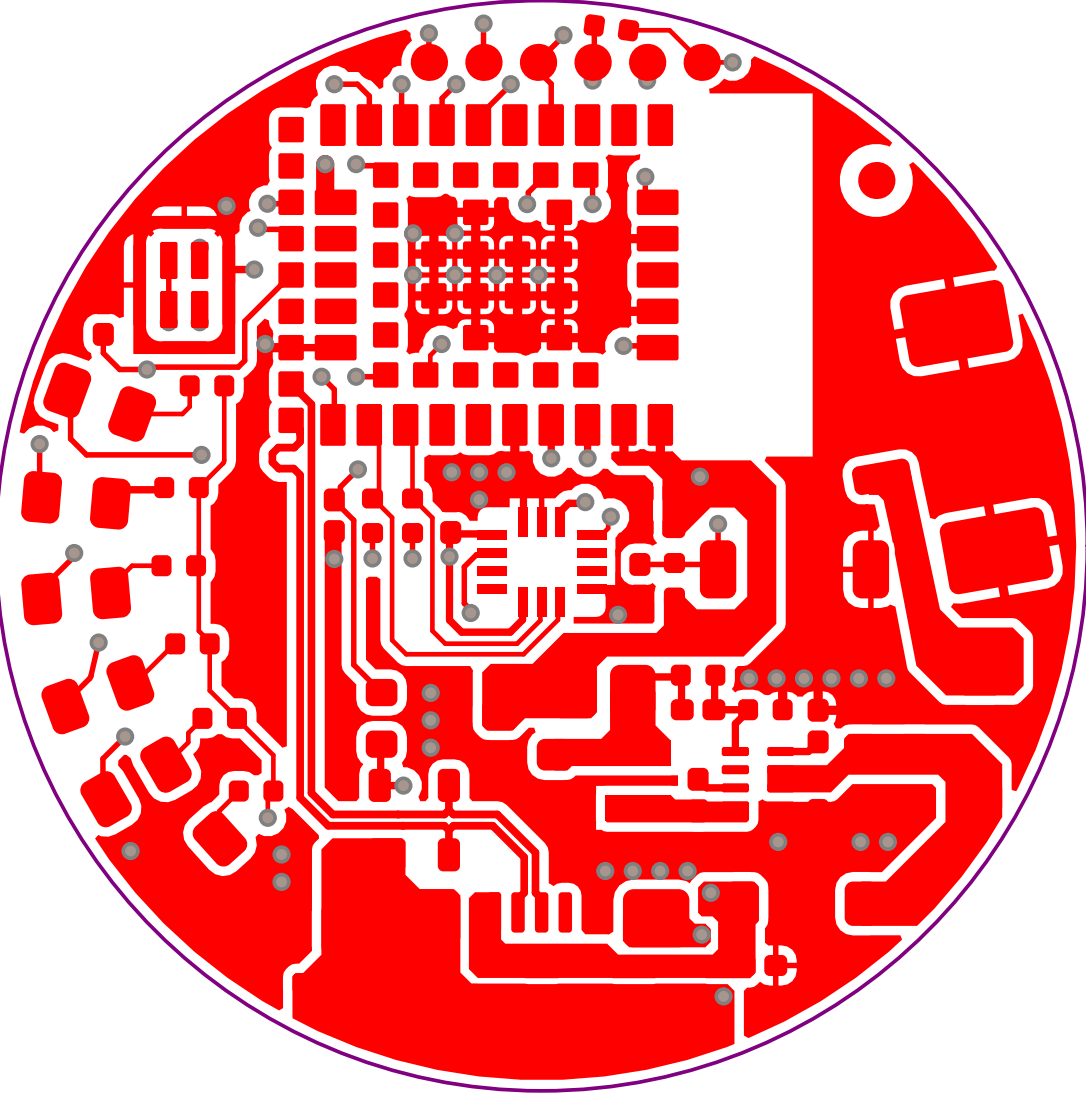
\includegraphics[width=0.5\textwidth]{images/pcd_dong_top.png}
        \label{fig:pcb_dong_top}
        \caption{Lớp đồng trên}

    \end{subfigure}
    \hfill
    \begin{subfigure}[b]{0.48\textwidth}
        \centering
        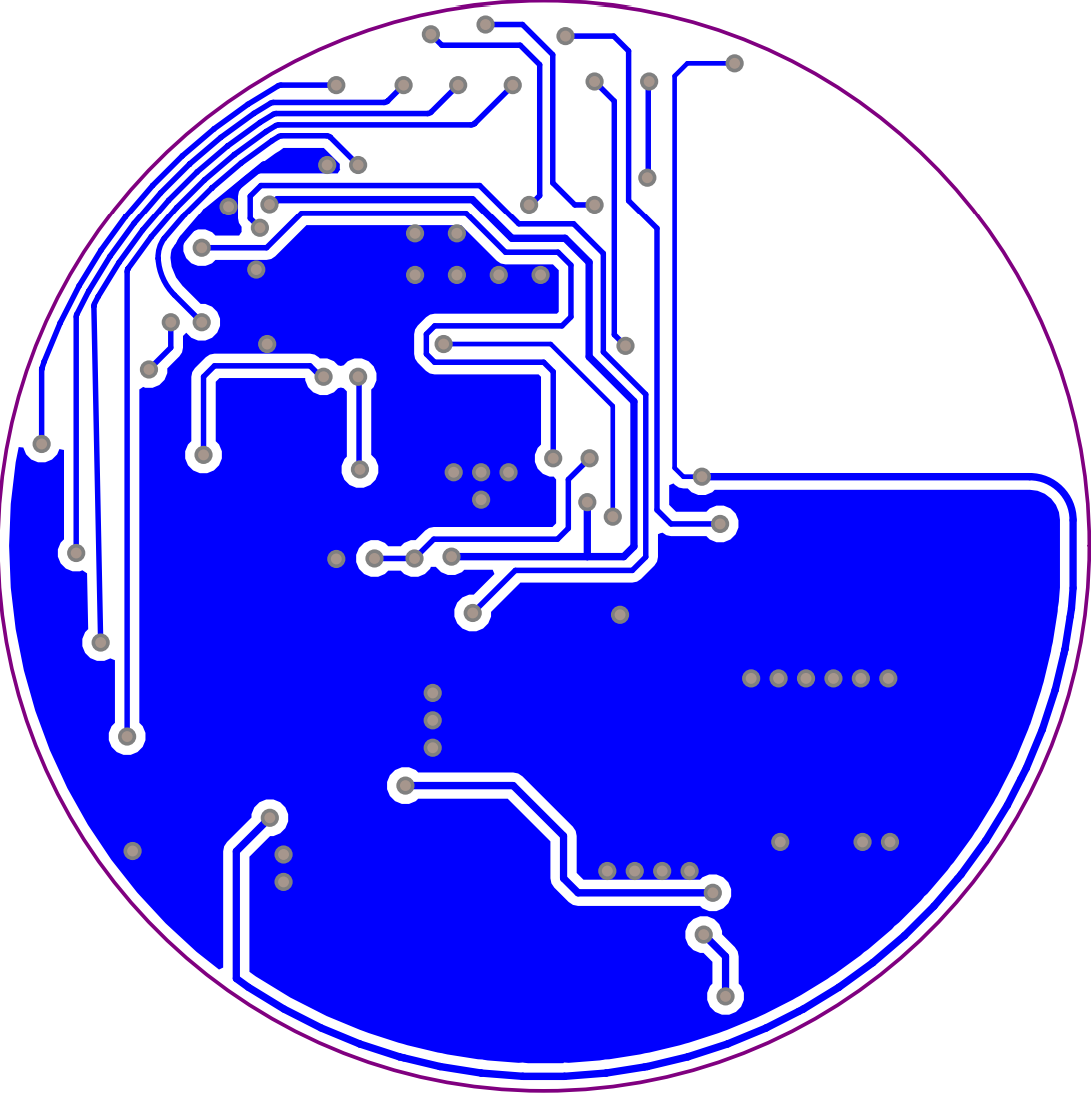
\includegraphics[width=0.5\textwidth]{images/pcb_dong_bottom.png}
        \label{fig:pcb_dong_bottom}
        \caption{Lớp đồng dưới}

    \end{subfigure}
    \centering
    \begin{subfigure}[b]{0.48\textwidth}
        \centering
        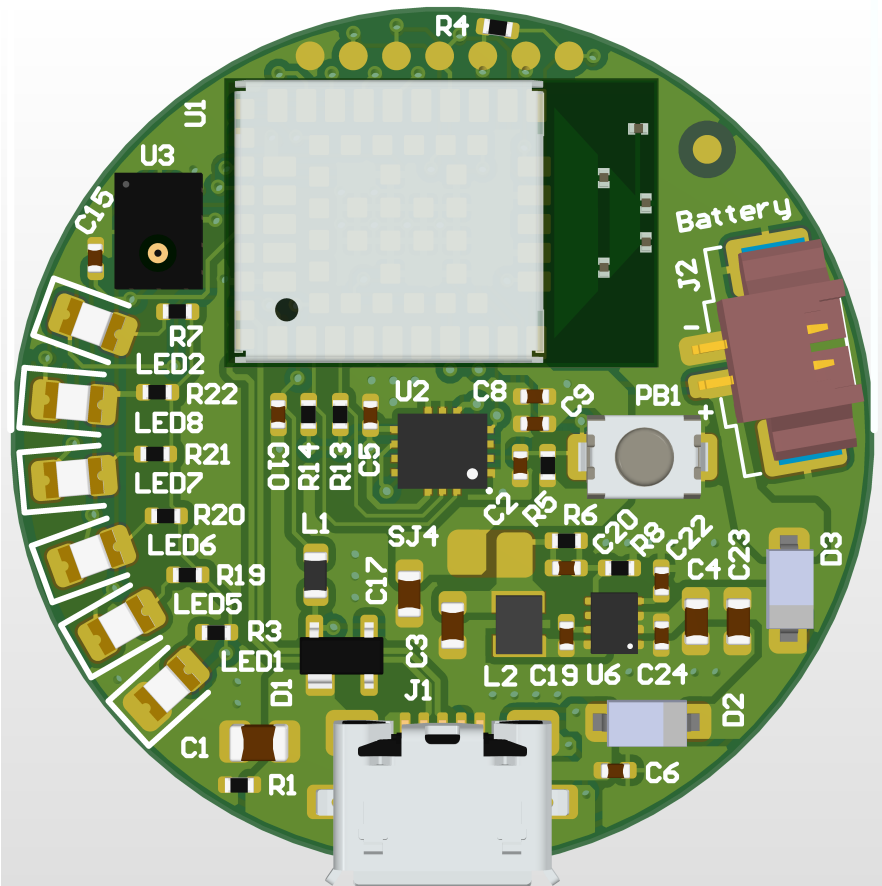
\includegraphics[width=0.5\textwidth]{images/pcb_3d_top.png}
        \caption{Mô hình 3D mặt trên}
    \end{subfigure}
    \hfill
    \begin{subfigure}[b]{0.48\textwidth}
        \centering
        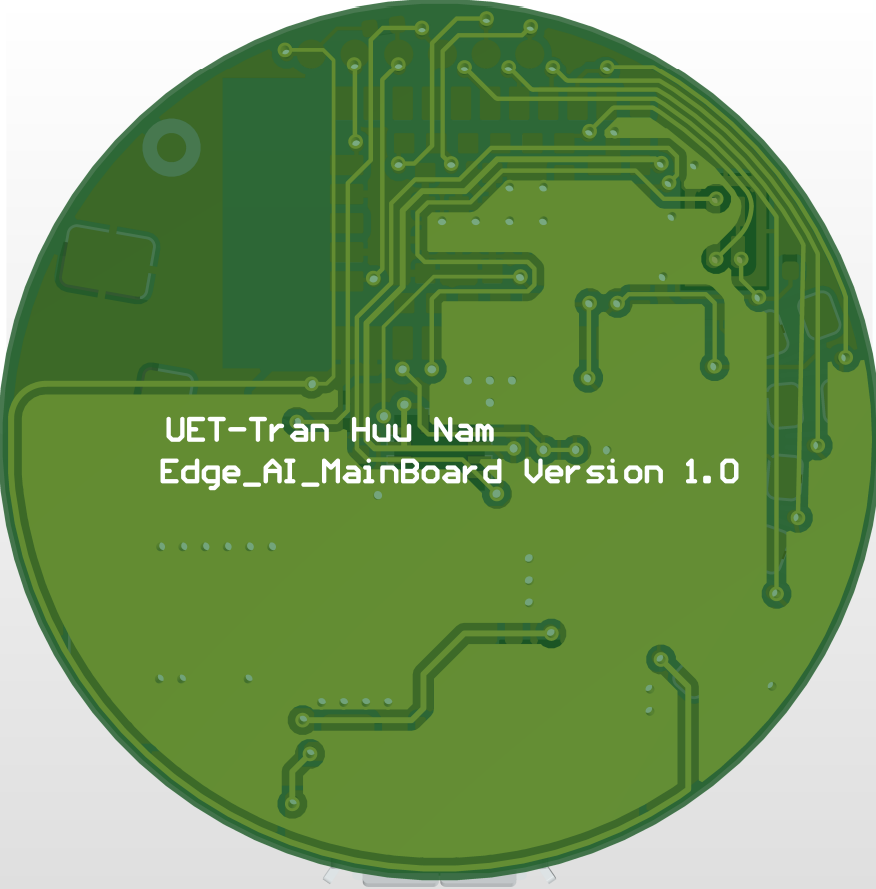
\includegraphics[width=0.5\textwidth]{images/pcb_3d_bottom.png}
        \caption{Mô hình 3D mặt dưới}

    \end{subfigure}
    \caption{Minh họa bố trí mạch in và mô hình 3D}
    \label{fig:pcb_3d}
\end{figure}

\newpage

\section{Hệ thống phần mềm}
Phần này trình bày tổng quan kiến trúc hệ thống phần mềm bao gồm: lập trình
phần cứng để đọc giá trị cảm biến, cấu hình BLE; phát triển ứng dụng di động
làm cầu nối giữa phần cứng và hệ thống đám mây, cùng với máy chủ và cơ sở dữ
liệu lưu trữ dữ liệu. Nội dung cũng đề cập đến các yêu cầu chức năng, phi chức
năng và thiết kế hệ thống ở mức cao nhằm đảm bảo khả năng triển khai thực tế và
mở rộng trong tương lai.

\subsection{Lập trình phần cứng}

Trong phần này sẽ trình bày chi tiết các bước: cấu hình vi điều khiển và cảm
biến, cấu hình BLE và lọc nhiễu bằng bộ lọc Kalman.

\subsection{Phần mềm thu thập, lưu trữ}

Phần mềm trong nghiên cứu này không chỉ là công cụ trực quan hoá dữ liệu cảm
biến, mà còn được thiết kế như một mắt xích trọng yếu trong quy trình từ thu
thập, truyền tải. Cách tiếp cận này đảm bảo rằng dữ liệu thu nhận từ môi trường
thực tế được xử lý nhất quán, có khả năng tái sử dụng và dễ dàng tích hợp với
các hệ thống khác.

\begin{figure}[H]
    \centering
    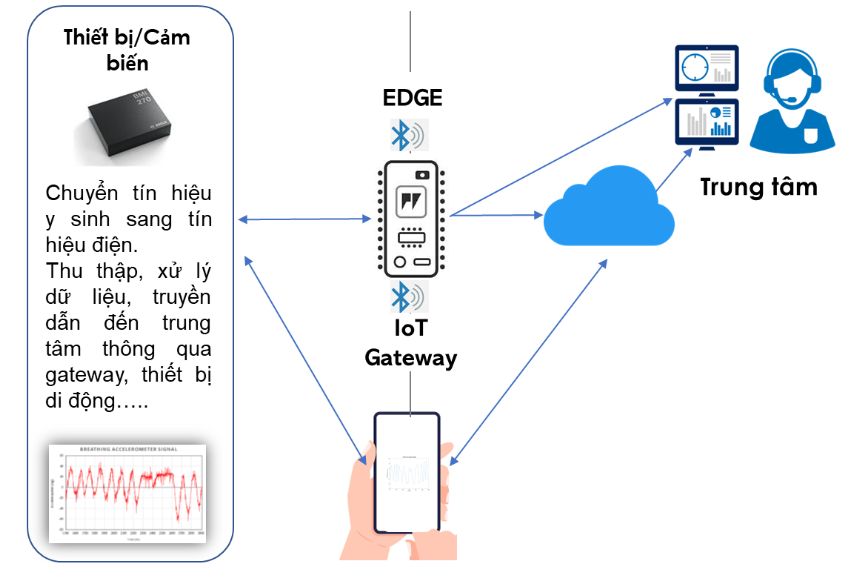
\includegraphics[width=1\textwidth]{images/architecture_software.png}
    \caption{Kiến trúc tổng thể của hệ thống}
    \label{fig:architecture_software}
\end{figure}

\subsubsection{Ứng dụng di dộng}
Được coi như một cổng kết nối trung gian trong mô hình điện toán đám mây
có nhiệm vụ gom các tín hiệu từ cảm biến gia tốc, hiển thị chúng theo thời gian thực và chuyển
lên máy chủ đám mây.
Dựa vào mục tiêu nghiên cứu, luận văn làm rõ các yêu cầu chức năng và phi chức năng.

\subsubsection{Máy chủ đám mây}

Máy chủ trung tâm có nhiệm vụ tiếp nhận và phản hồi các yêu cầu từ ứng dụng di
động. Đi kèm với cơ sở dữ liệu có nhiệm vụ lưu trữ dữ liệu liên quan đến người
dùng và dữ liệu của cảm biến. Vì vậy, kết hợp cả NoSQL (MongoDB) và SQL
(Postgres) sẽ là phương pháp tối ưu nhất và được nhiều dự án thực tế lựa chọn.
MongoDB thể hiện ưu thế vượt trội nhờ mô hình lưu trữ dạng tài liệu, cho phép
linh hoạt mở rộng cấu trúc dữ liệu mà không cần định nghĩa cột hàng cố định.
Ngược lại, sử dụng PostgreSQL nhằm quản lý các dữ liệu có cấu trúc ổn định và
đòi hỏi tính toàn vẹn cao. Ngoài ra, phục vụ mục đích lưu các tệp dữ liệu như
ảnh, hệ thống sử dụng một Object Storage là Minio.

\begin{figure}[H]
    \centering
    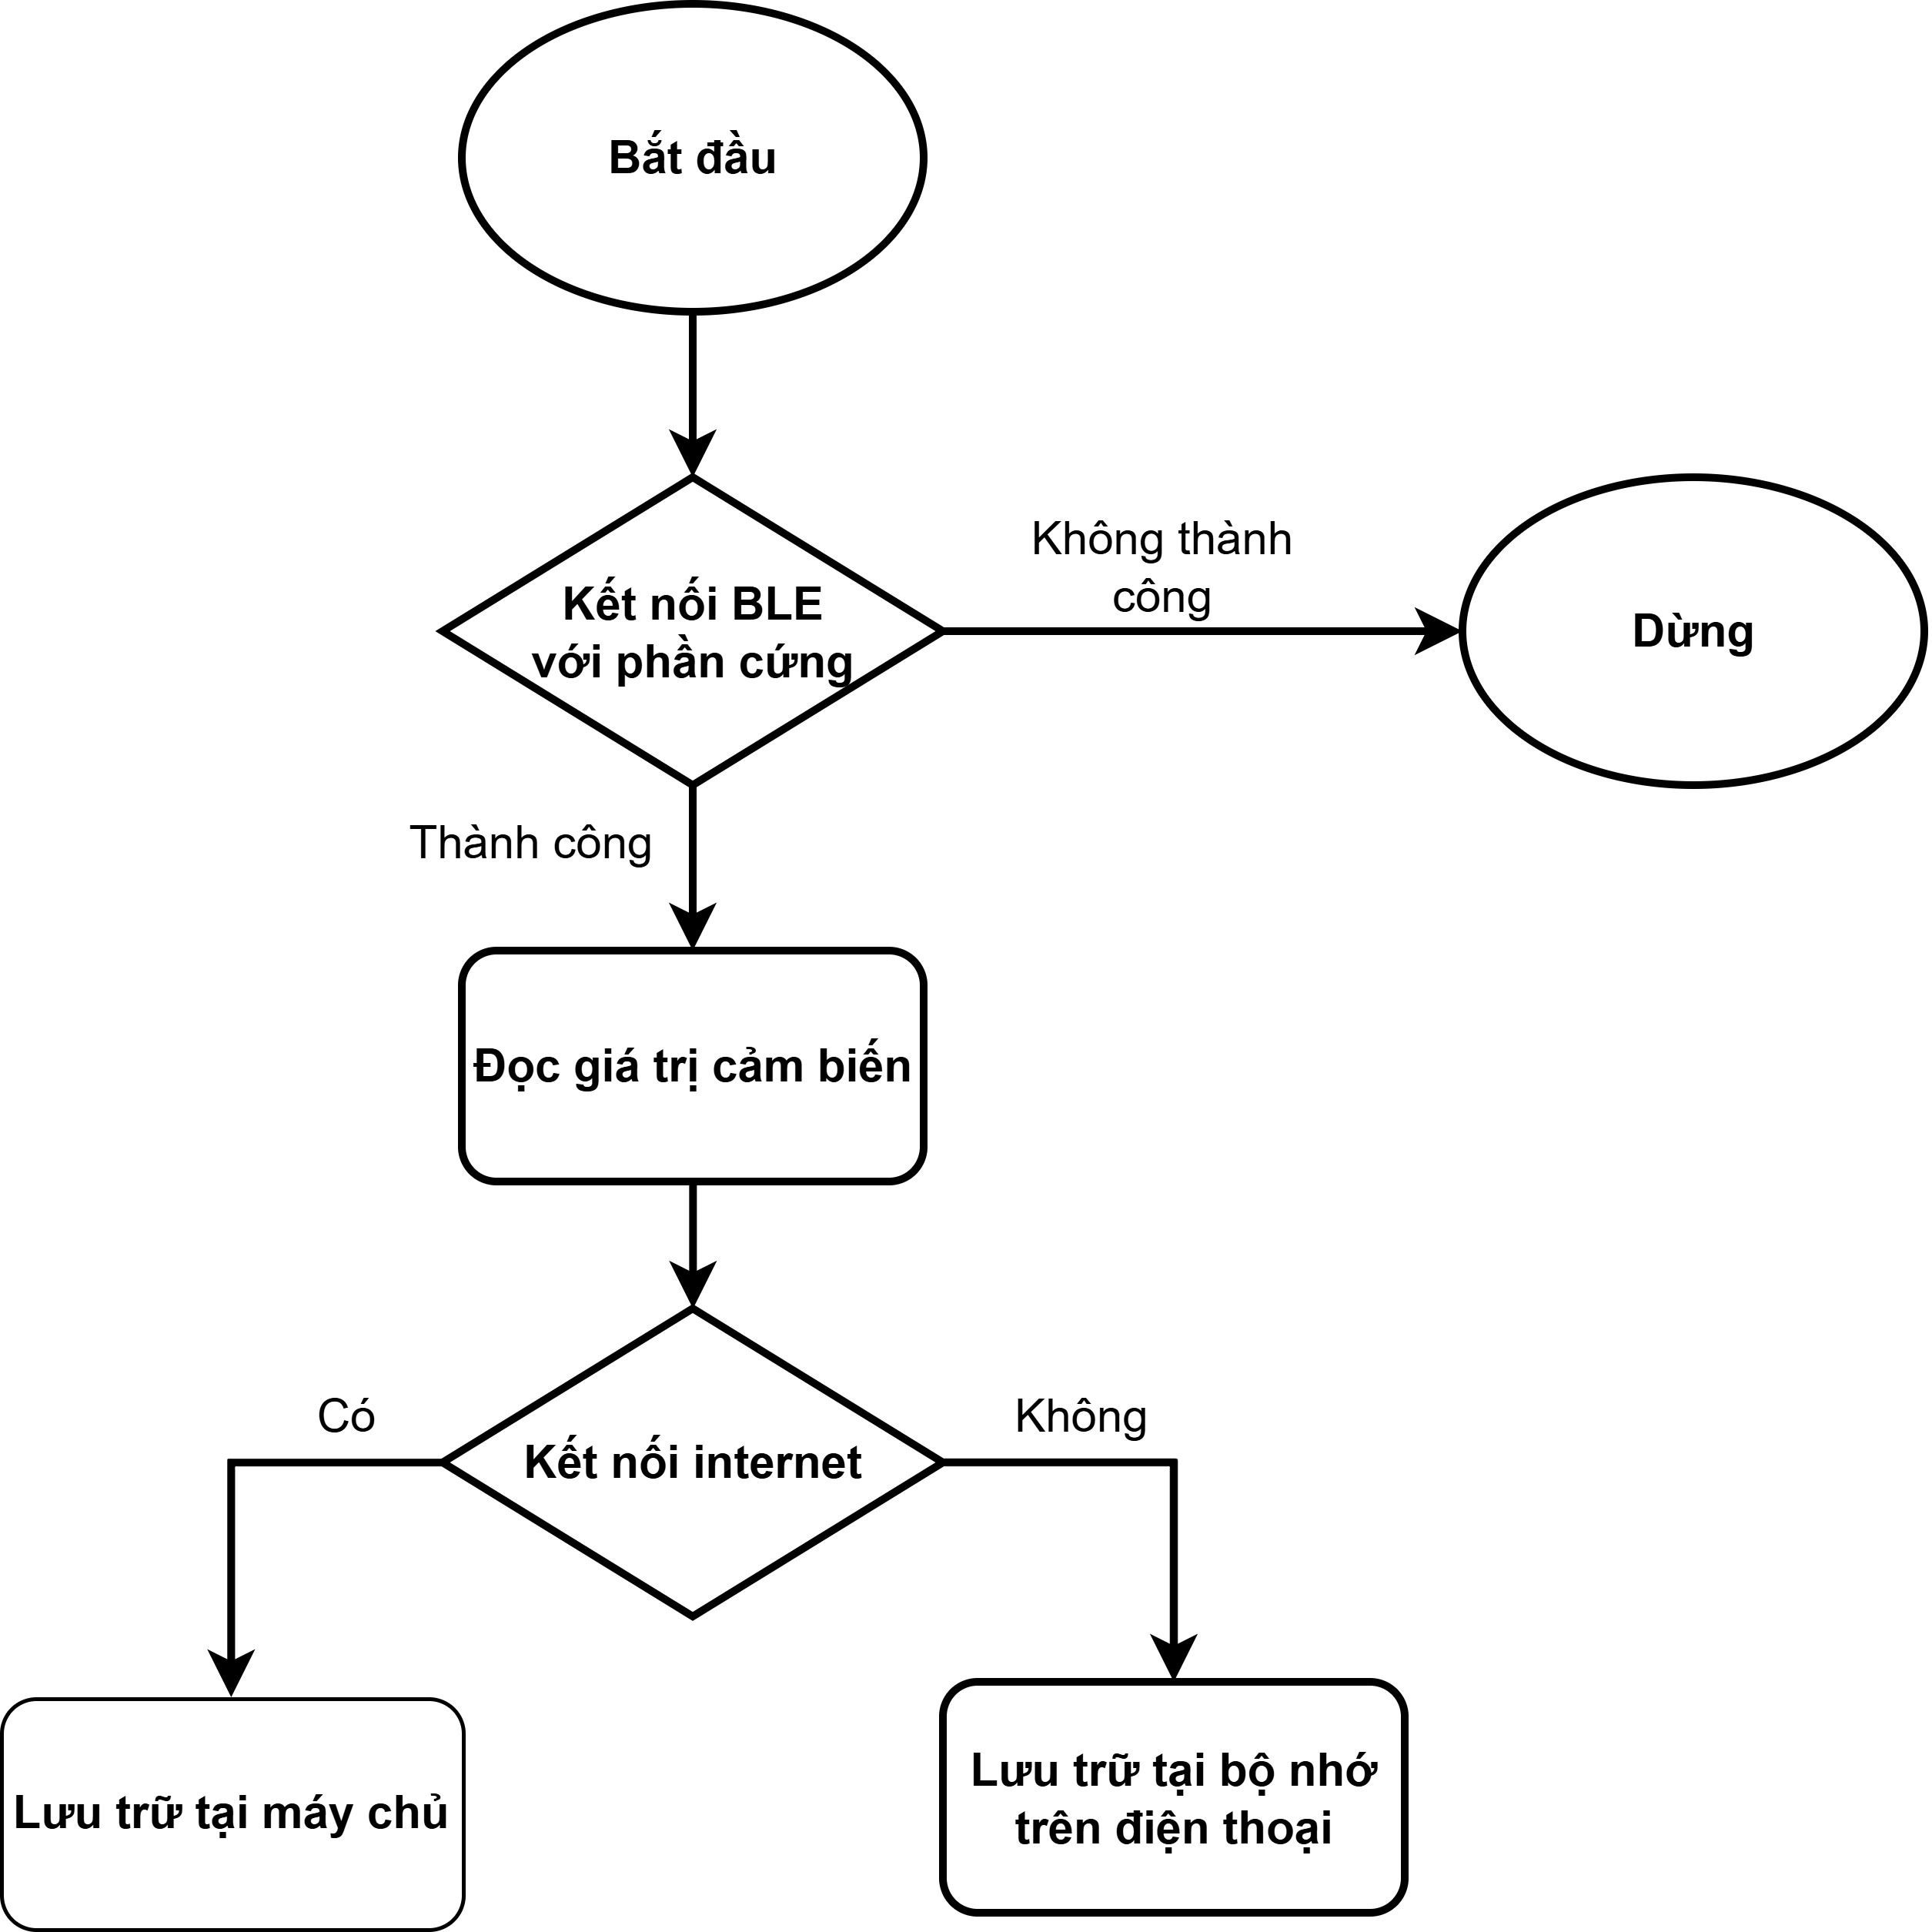
\includegraphics[width=0.8\textwidth]{images/master.2025-chuẩn-Trang-3 (1).jpg}
    \caption{Lưu đồ thuật toán lưu trữ dữ liệu cảm biến}
    \label{flow_http}
\end{figure}

Lưu đồ thuật toán lưu trữ dữ liệu được thể hiện trong Hình~\ref{flow_http}, bao
gồm hai nhánh xử lý. \textit{(i)} Khi người dùng không có kết nối mạng, dữ liệu
sẽ được lưu trữ tạo tại ngay bộ nhớ của điện thoại. \textit{(ii)} Khi người
dùng đã đăng nhập và có Internet, khi nhận đủ 1000 mẫu, ứng dụng di động sẽ đẩy
gói đó lên máy chủ. Khi này, máy chủ sẽ mở các API để có thể lấy dữ liệu (giá
trị cảm biến, thời gian và thông tin của người thực hiện) định dạng CSV để sử
dụng cho bài toán học máy.

\subsection{Học máy trong phân loại tư thế ngủ}

Tổng quan về các bước xây dựng hệ thống học máy cho bài toán phân loại tư thế
ngủ đã được trình bày tại Chương~\ref{chapter:1-introduction}. Sau khi đánh
giá, 4 mô hình học máy truyền thống là rừng ngẫu nhiên (Random forest - RF),
máy vec-tơ hỗ trợ (Support vector machine - SVM), hồi quy Logistic (Logistic
regression - LR), thuật toán tăng cường Gradient Boosting (GB) và một mô hình
mạng nơ-ron nhân tạo (Artificial Neural Network - ANN), được lựa chọn.
